\subsection{Object Selection}

Jets are separated into two groups based on their kinematics: 
\begin{description}
	\item[\textit{Central} jets:] $|\eta| < 2.5,\ \pt \ge 40\ \GeV$ -  these jets are used for triggering and will form  Higgs-candidates;
	\item[\textit{Forward} jets:] $|\eta| \ge 2.5,\ \pt \ge 30\ \GeV$ - these extra jets are used to improve the acceptance of jets produced in the vector boson fusion production process.
\end{description}

\subsubsection{\Pqb-jets Selection}
\label{sec:sel-btag}

In order to maximize sensitivity, events are selected and categorized based on the number of \Pqb-tagged \textit{central} jets. 
The \Pqb-tagging algorithm used, DL1r, is described in \Sect{\ref{subsec:ftag}}. 

\paragraph{Ordering and selection} For the jets that form our Higgs Candidates, we take the four leading \Pqb-tagged jets. In events with less than four \Pqb-jets, the extra jets are selected as the highest $p_T$ jets from the pool of \textit{central} jets which failed the initial \Pqb-tag requirement.

\paragraph{\Pqb-tag Requirements} The \Pqb-tag selection for ggF and VBF signals is to require \textbf{at least 4 central jets with DL1r 77\% WP}. Events with two \bjets are classified as 2b events and are used for deriving the data-driven background estimate described in \Sect{\ref{sec:bkgdestimation}}. We also define a systematic on our background estimation using events with 3 \Pqb-tags, and the corresponding \Pqb-tag categories used in this analysis are summarized in table \ref{tab:b-tag-cat}.

\begin{table}[!htbp]
	\centering
	  \begin{tabularx}{\textwidth}{l|X|l}
	  Notation     & Definition & Usage \\
	  \toprule
	  2b    & Exactly two central jets tagged with DL1r 77\% WP & Background estimation \\ \hline
	  3b1f  & Exactly three central jets tagged with DL1r 77\% WP and no central jets passing the 85\% WP (the leading \pT non-\Pqb-jet is taken for the last Higgs Candidate jet) & Background estimate systematic \\ \hline
	  4b    & At least four central jets tagged with DL1r 77\% WP & Signal region (ggF and VBF) \\
	  \bottomrule
	  \end{tabularx}
	\caption{Different analysis definitions based on number of \Pqb-tags.}
	\label{tab:b-tag-cat}
  \end{table}%

  \paragraph{Accuracy} The Higgs jet selection accuracy is defined as the probability that all four \Pqb-jets in the event are matched to the truth \Pqb-quarks using a $\Delta R$ < 0.3 matching criterion, and is shown is \Fig{\ref{fig:jetSel-4b}}.
  The jet selection accuracy is 74\% for the ggF selection with \%-level variations across the \kl values of interest. 
  This means that there is a \SI{74}{\%} chance the selected four \Pqb-jets are coming from the real Higgs decayed \Pqb-quarks. This accuracy loss is dominated by events where one of the \Pqb-quarks is out of acceptance. 
  The 4b VBF selection has an average \Pqb-quark selection accuracy of 85\% and 90\% for the respective \kl and \kvv signal samples.
  The dependency on \kl and/or \kvv is likely due to the positive dependence of the \Pqb-tagging efficiency on the \Pqb-jet \pt: harder signals lead to higher \Pqb-tagging efficiency therefore higher Higgs jet selection accuracies. 
  \Fig{\ref{fig:jetSel-mhh}} shows the truth \mhh distributions and the reconstructed histograms for the cases where we did or did not selected the correct jets for the ggF and VBF selections at a few signal points. As discussed above, we are less likely to select the correct jets for lower \mhh, and also the signal shapes for the \kl and \kvv variations are quite different, this is entirely due to the underlying \mhh distribution.
    
  \begin{figure}[hbt]
	  \centering
	  \subfloat[Jet selection accuracy vs \kl]{
			   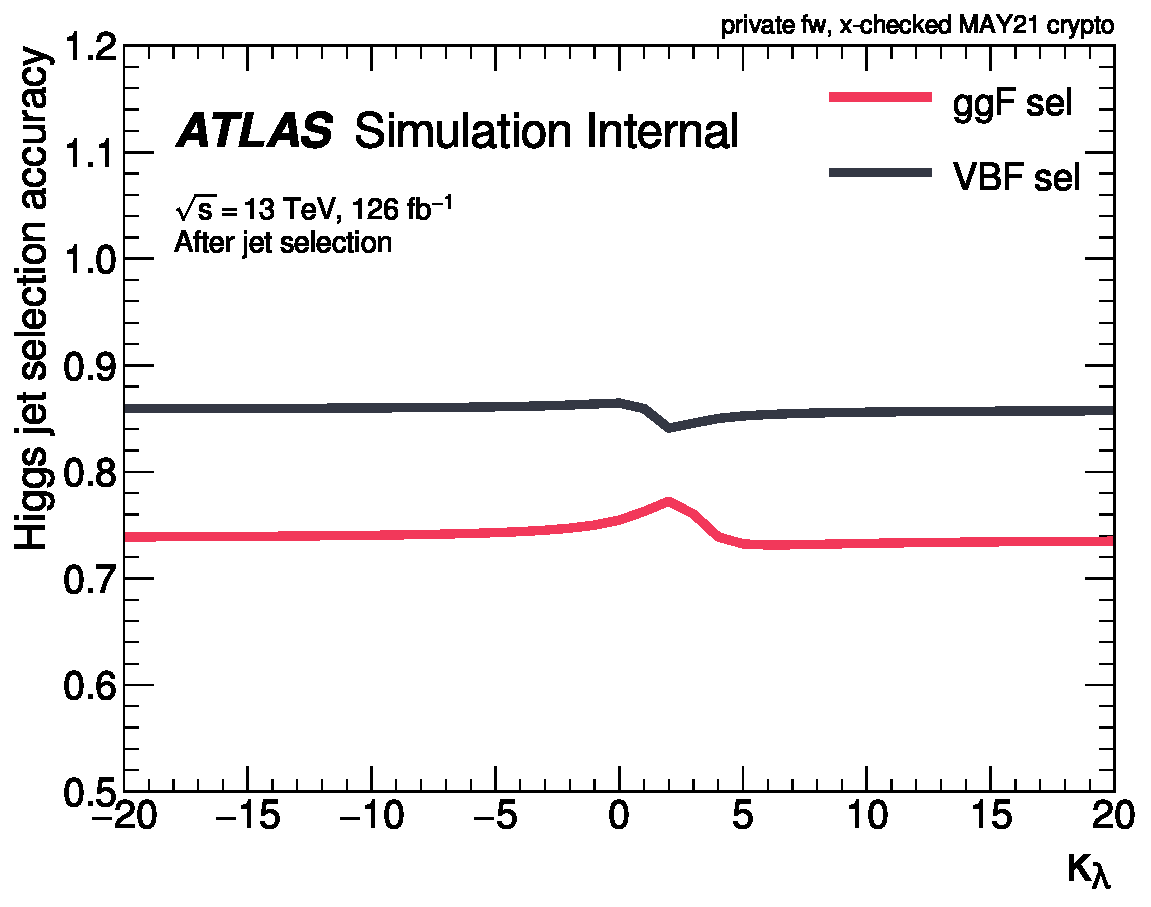
\includegraphics[width=0.4\textwidth]{figures/nr-int-note/selection/V2/jetSel_kl_4b_only.pdf}
		  \label{fig:jetSel-kl}
	  }
	  \subfloat[Jet selection accuracy vs $\kappa_{2V}$]{
			   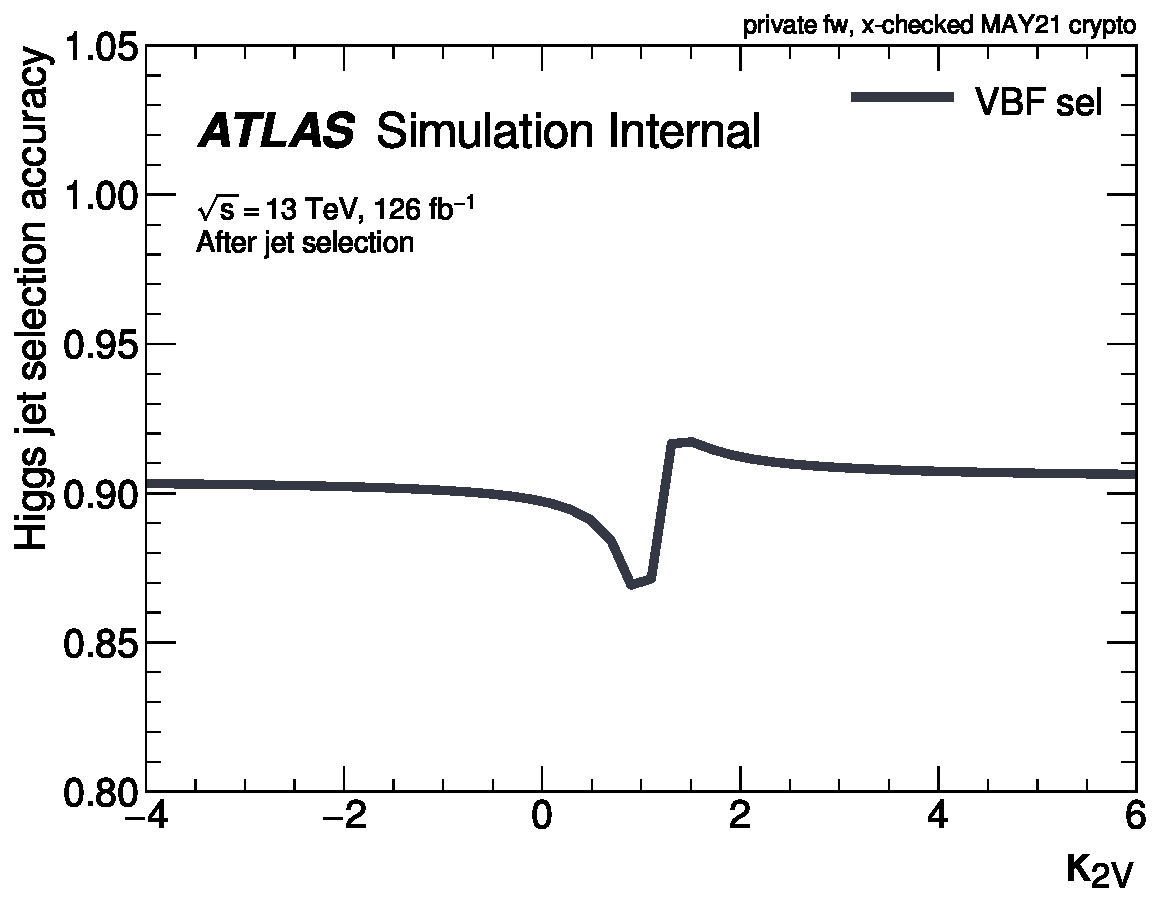
\includegraphics[width=0.4\textwidth]{figures/nr-int-note/selection/V2/jetSel_k2V.pdf} 
		  \label{fig:jetSel-k2V}
	  }
	  \caption{The jet selection accuracy as a function of \kl and \kvv.}
	  \label{fig:jetSel-4b}
  \end{figure}

  \begin{figure}[hbt]
	  \centering
	  \subfloat[ggF signals]{
			   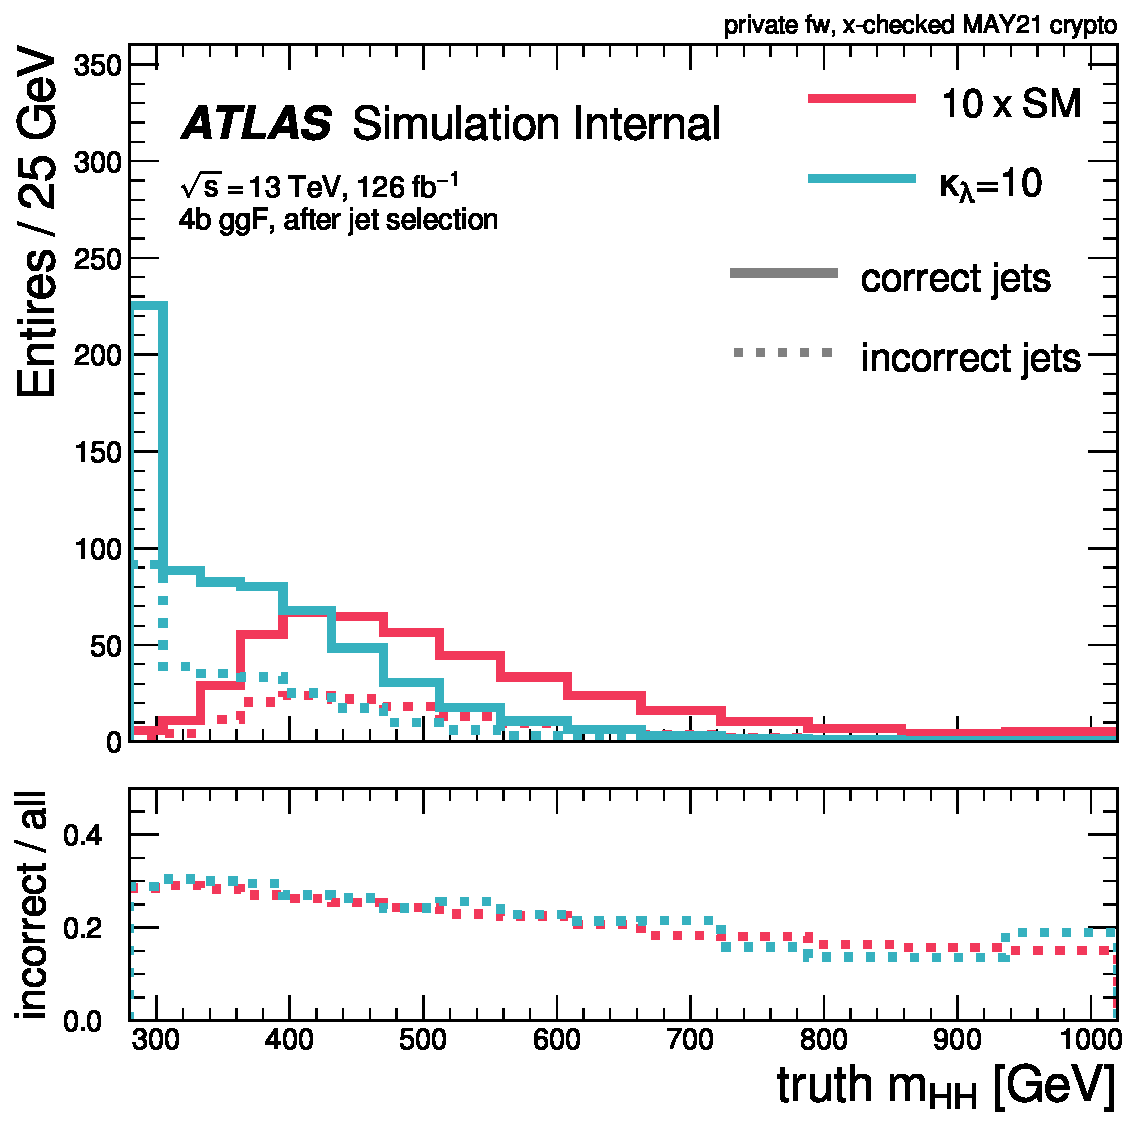
\includegraphics[width=0.4\textwidth]{figures/nr-int-note/selection/V2/truth_mhh_4b_jetSelAcc.pdf}
		  \label{fig:jetSel-kl}
	  }
	  \subfloat[VBF signals]{
			   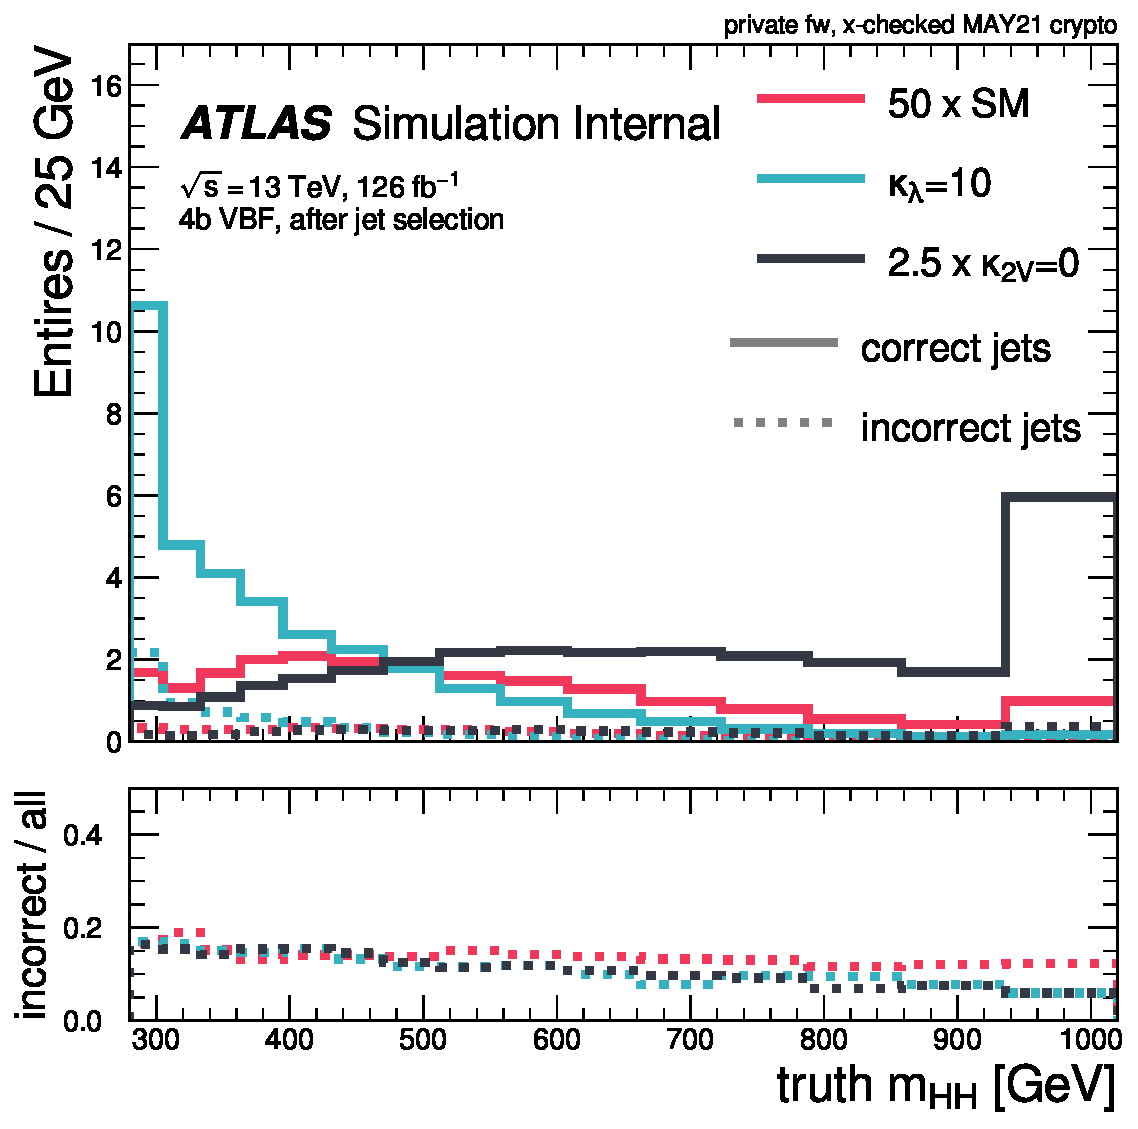
\includegraphics[width=0.4\textwidth]{figures/nr-int-note/selection/V2/truth_mhh_3b1l_jetSelAcc_vbf.pdf} 
		  \label{fig:jetSel-k2V}
	  }
	  \caption{Truth \mhh distributions for correctly and incorrectly selected jets, for ggF (a) and VBF (b) signals.}
	  \label{fig:jetSel-mhh}
  \end{figure}